%---------------------------------------------------------------------------
% MBS Benchmark A01: Simple Pendulum
%---------------------------------------------------------------------------
%
% LaTeX Template: Jacobs Landscape Poster
% Created by:
% Computational Physics and Biophysics Group, Jacobs University
% https://teamwork.jacobs-university.de:8443/confluence/display/CoPandBiG/LaTeX+Poster

\documentclass[final]{beamer}

\usepackage[scale=1.24]{beamerposter} % Use the beamerposter package for laying out the poster

\usetheme{confposter} % Use the confposter theme supplied with this template

\setbeamercolor{block title}{fg=ngreen,bg=white} % Colors of the block titles
\setbeamercolor{block body}{fg=black,bg=white} % Colors of the body of blocks
\setbeamercolor{block alerted title}{fg=white,bg=dblue!70} % Colors of the highlighted block titles
\setbeamercolor{block alerted body}{fg=black,bg=dblue!10} % Colors of the body of highlighted blocks
% Many more colors are available for use in beamerthemeconfposter.sty

%-----------------------------------------------------------
% Define the column widths and overall poster size
% To set effective sepwid, onecolwid and twocolwid values, first choose how many columns you want and how much separation you want between columns
% In this template, the separation width chosen is 0.024 of the paper width and a 4-column layout
% onecolwid should therefore be (1-(# of columns+1)*sepwid)/# of columns e.g. (1-(4+1)*0.024)/4 = 0.22
% Set twocolwid to be (2*onecolwid)+sepwid = 0.464
% Set threecolwid to be (3*onecolwid)+2*sepwid = 0.708

\newlength{\sepwid}
\newlength{\onecolwid}
\newlength{\twocolwid}
\newlength{\threecolwid}
\setlength{\paperwidth}{48in} % A0 width: 46.8in
\setlength{\paperheight}{36in} % A0 height: 33.1in
\setlength{\sepwid}{0.024\paperwidth} % Separation width (white space) between columns
\setlength{\onecolwid}{0.301\paperwidth} % Width of one column
\setlength{\twocolwid}{0.602\paperwidth} % Width of two columns
\setlength{\threecolwid}{0.903\paperwidth} % Width of three columns
\setlength{\topmargin}{-0.5in} % Reduce the top margin size
%-----------------------------------------------------------

\usepackage{graphicx}  % Required for including images
\graphicspath{{../MBSfigures/}}
\usepackage{booktabs} % Top and bottom rules for tables

\usepackage{subfigure}
\usepackage{multirow}
\usepackage{siunitx}
%----------------------------------------------------------------------------------------
%	TITLE SECTION 
%----------------------------------------------------------------------------------------

\title{MBS Benchmark A02: N Four-Bar Mechanism} % Poster title




%----------------------------------------------------------------------------------------

\begin{document}

%\addtobeamertemplate{block end}{}{\vspace*{2ex}} % White space under blocks
%\addtobeamertemplate{block alerted end}{}{\vspace*{2ex}} % White space under highlighted (alert) blocks

\setlength{\belowcaptionskip}{2ex} % White space under figures
\setlength\belowdisplayshortskip{2ex} % White space under equations

\begin{frame}[t] % The whole poster is enclosed in one beamer frame

\begin{columns}[t] % The whole poster consists of three major columns, the second of which is split into two columns twice - the [t] option aligns each column's content to the top

\begin{column}{\sepwid}\end{column} % Empty spacer column

\begin{column}{\twocolwid} % The first column

%----------------------------------------------------------------------------------------
%	OBJECTIVES
%----------------------------------------------------------------------------------------

\begin{alertblock}{Benchmark Objective}
The NMS benchmark problem \textbf{A02} is a common example of a mechanism which undergoes singular configuration~\cite{gonzalez2006benchmarking}.
\end{alertblock}

%----------------------------------------------------------------------------------------
%    BENCHMARK DESCRIPTION
%----------------------------------------------------------------------------------------


\begin{columns}[t, totalwidth=\twocolwid]

\begin{column}{0.95\onecolwid}
\begin{block}{Benchmark Description}
N four-bar mechanism (Fig.~\ref{FIG:NFourBarMechanism}) is a common example of a mechanism which undergoes singular configuration.
%
The system has N four-bar windows composed of 2N+1 links. It is an extension of the two four-bar mechanism proposed in~\cite{bayo1994singularity}.
%
When the mechanism reaches the horizontal position, the number of the degrees of freedom instantaneously increase from 1 to N+1.
%
Gravity is on the negative $y$ direction.

Tab.~\ref{TAB:SystemProperties} reports the system properties.
\end{block}


\begin{figure}[h]
\centering
\label{FIG:N-FourBar}
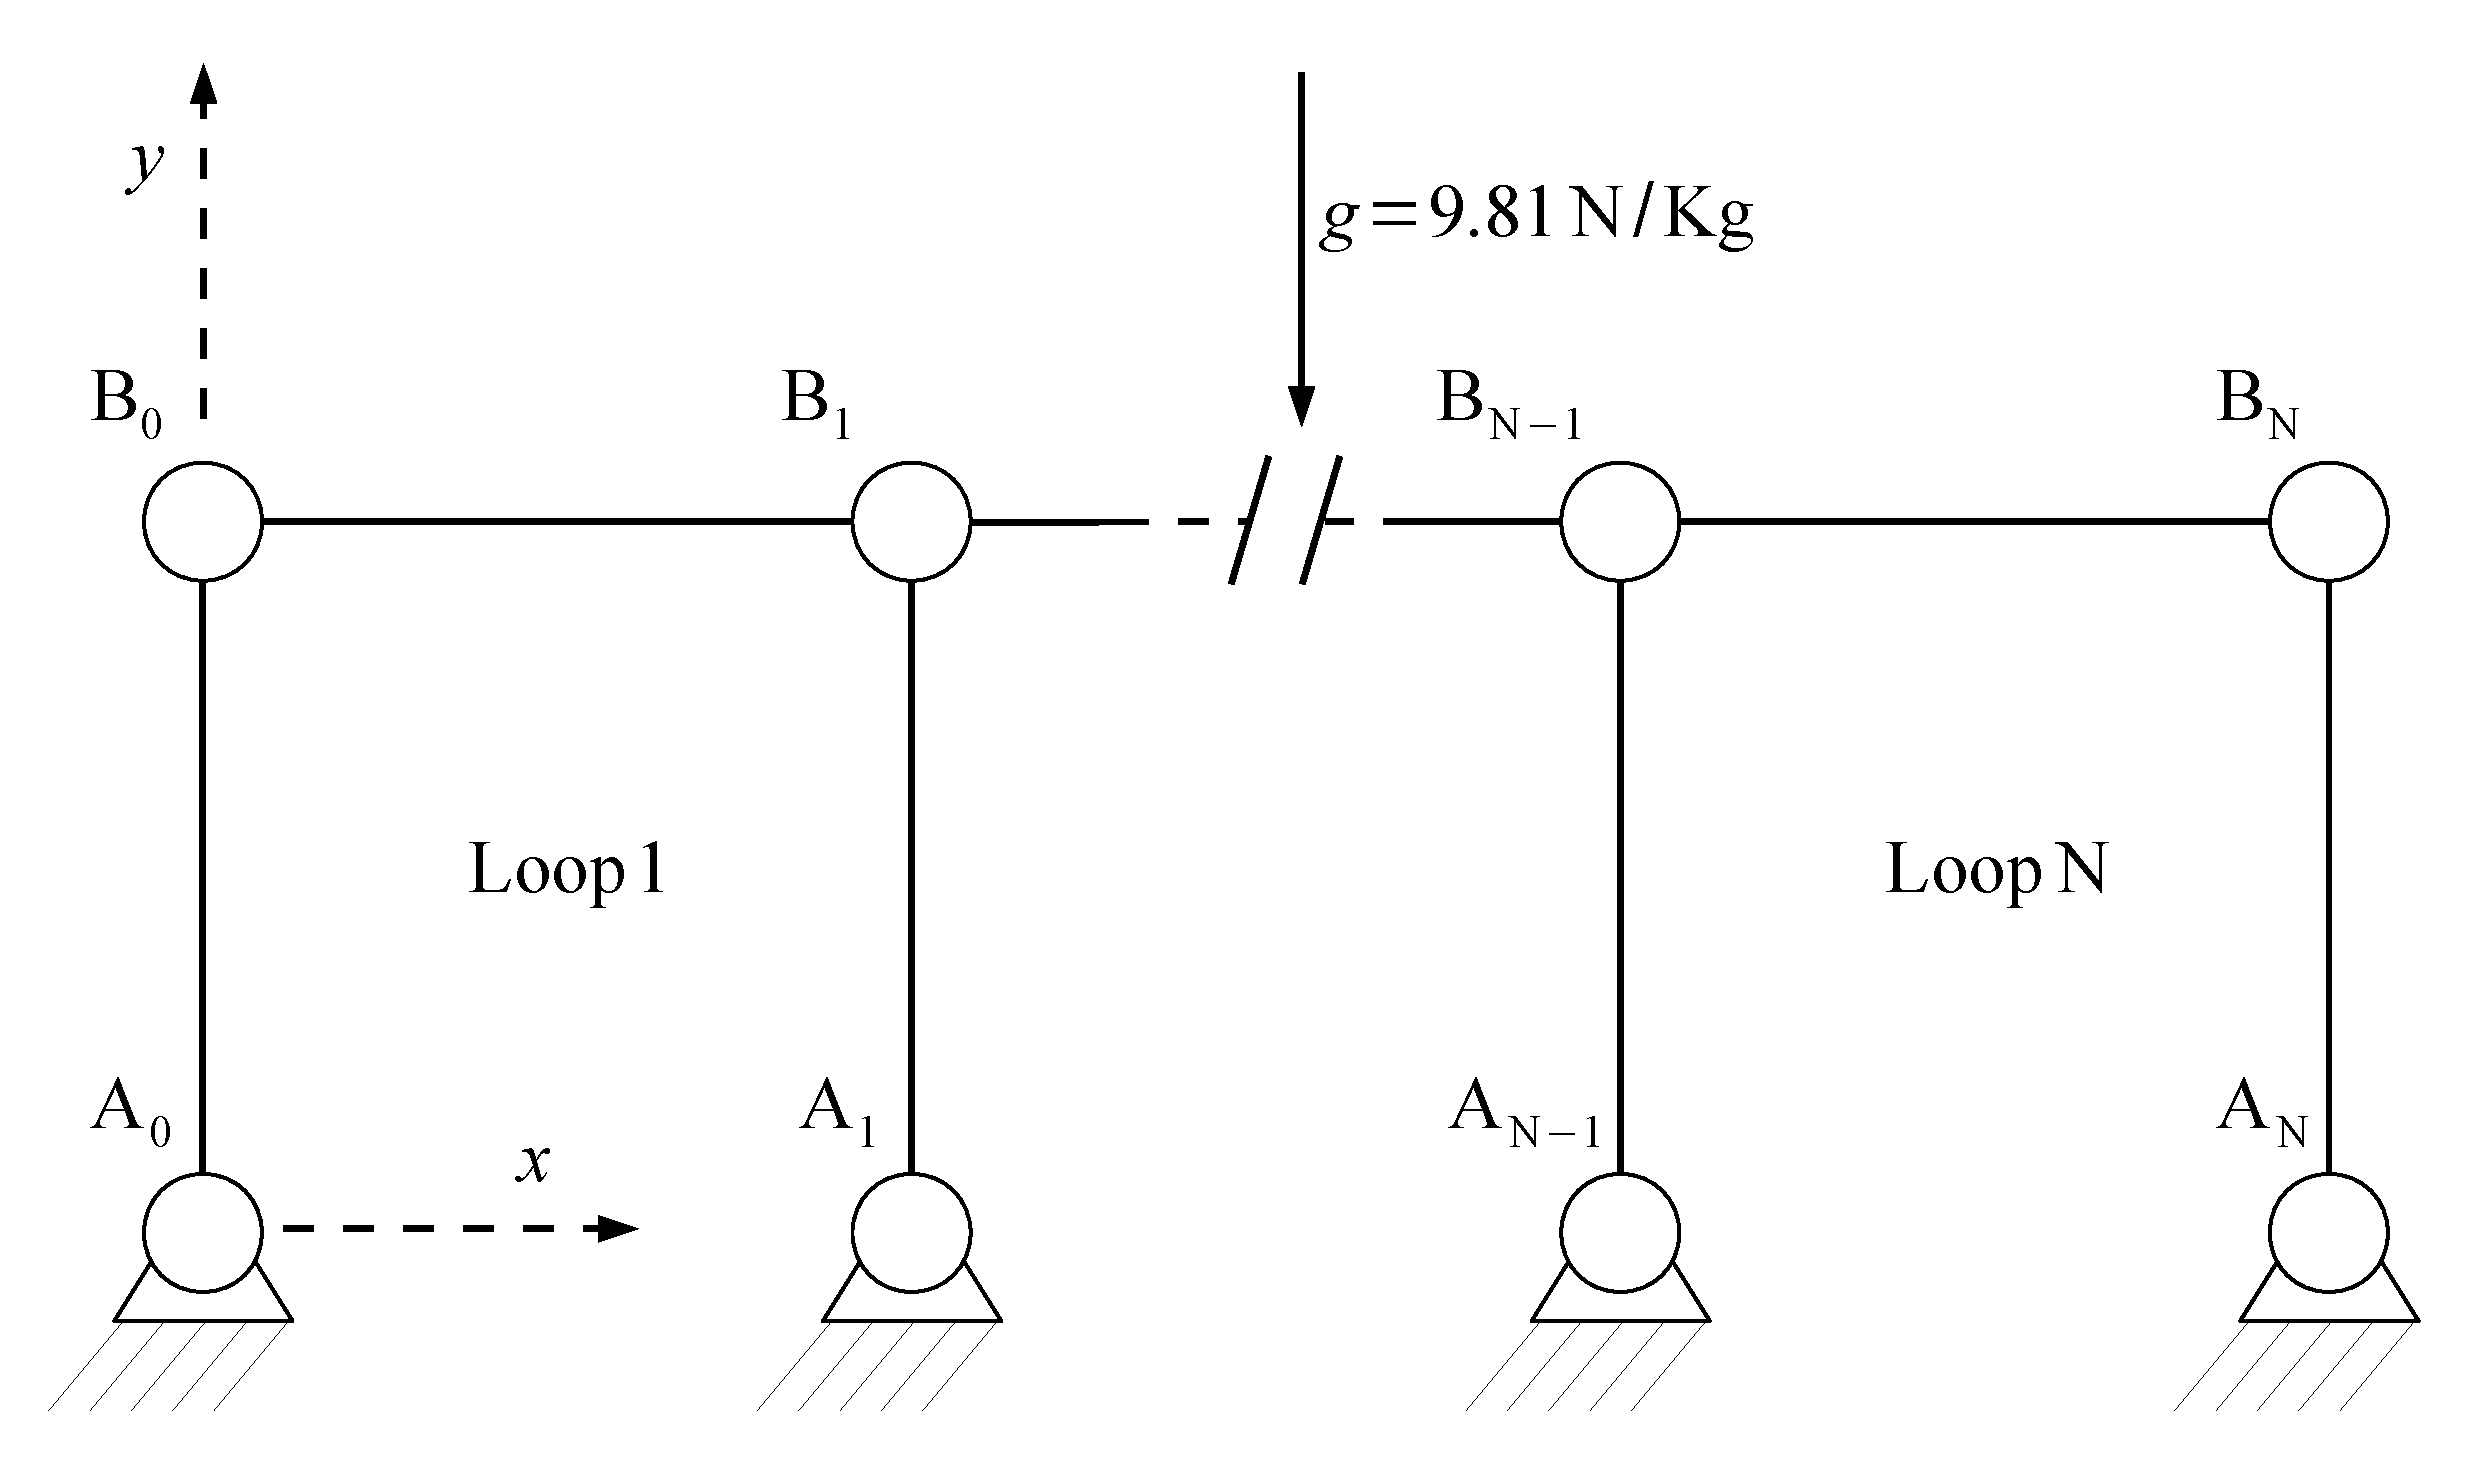
\includegraphics[width=0.95\onecolwid] {2MBS_N-FourBar.pdf}
\caption{N four-bar mechanism sketch.}
\label{FIG:NFourBarMechanism}
\end{figure}


\begin{large}
\begin{table}
\vspace{2ex}
\begin{tabular}[b]{ll}
%\multicolumn{2}{c}{\textbf{System Properties}}\\
\toprule
$N$ & 40\\
Link mass & $\SI{1.0}{\kilogram}$\\
Link length & $\SI{1.0}{\metre}$\\	
$\dot{B_{0}}x(0)$ & $\SI{1.0}{\metre / \second}$\\
\bottomrule
\end{tabular}
\label{TAB:SystemProperties}
\caption{System Properties and Configuration}
\end{table}
\end{large}

\end{column}

\begin{column}{0.95\onecolwid}


%----------------------------------------------------------------------------------------
%    RESULTS
%----------------------------------------------------------------------------------------


\begin{block}{Results}
The dynamic simulation of the \textbf{A02} benchmark was executed for \SI{20}{\second}.
The starting position of the simulation is shown in  Fig.~\ref{FIG:NFourBarMechanism} with an initial speed for the point $B_0$ in the positive x-direction of $\SI{1}{\metre \per \second}$. 
The objective of the simulation is to measure the displacement of $B_0$, and compare the results with the reference solution~\cite{gonzalez2006benchmarking}.

The simulation with OpenSim perfectly matches the reference values. Fig.~\ref{FIG:simulationPlot} shows a $\SI{10}{\second}$ simulation. 


\begin{figure}[h]
\centering
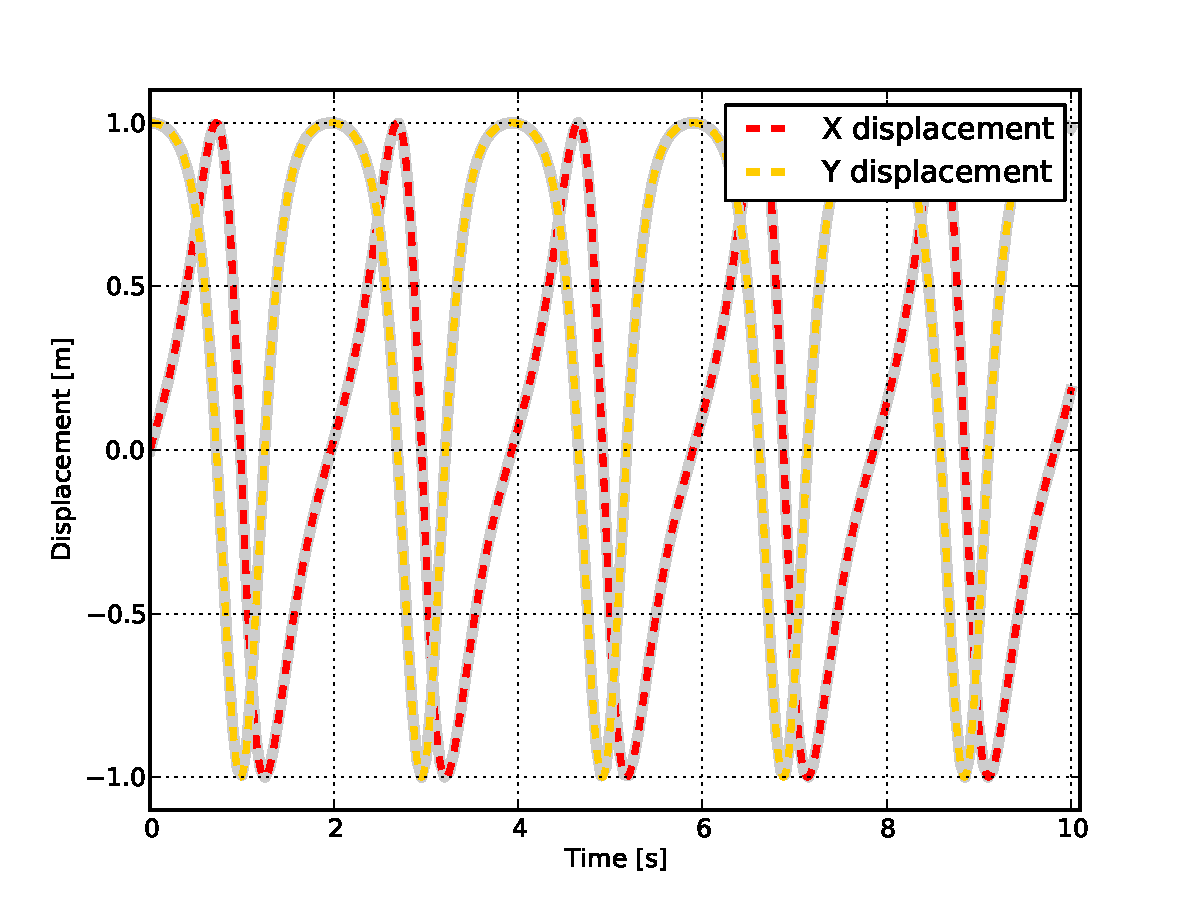
\includegraphics[width=0.95\onecolwid]{2MBS_PlotResults.pdf}
\caption{$B_{0}$ displacement in OpenSim simulation (dashed lines) and MBS benchmark reference values (gray lines). }
\label{FIG:simulationPlot}
\end{figure}

\end{block}

\end{column}
  

\end{columns}


\end{column}
\begin{column}{\onecolwid} % The third column


\begin{block}{Download}
\begin{itemize}
\item MBS Benchmark available at: \url{http://goo.gl/ySQ5me}
\item OpenSim implementation available at: \url{http://goo.gl/R9tl3z}
\item Videos of OpenSim simulation available at: \url{http://goo.gl/q4G2FZ}
\end{itemize}
\end{block}
\begin{block}{References}

\begin{thebibliography}{99}

\bibitem{gonzalez2006benchmarking} M. Gonz{\'a}lez, D. Dopico, U. Lugr{\'i}s, J. Cuadrado, \textit{``A benchmarking system for MBS simulation software: Problem standardization and performance measurement,''} 	in Multibody System Dyn., vol. 6, no.2,  2006, pp. 179--190.

\bibitem{bayo1994singularity} E. Bayo and A. Avello, \textit{``Singularity-Free Augmented Lagrangian Algorithms for Constrained Multibody Dynamics,''} Nonlinear Dyn., vol. 5, no. 2, 1994, pp. 209--231.

\end{thebibliography}

\end{block}

%----------------------------------------------------------------------------------------

\vspace{20cm}

\setbeamercolor{block alerted title}{fg=black,bg=norange} % Change the alert block title colors
\setbeamercolor{block alerted body}{fg=black,bg=white} % Change the alert block body colors


\begin{alertblock}{Contact Information}
Rehabilitation Engineering Group\newline Department of Management and Engineering\newline University of Padua

\begin{itemize}
\item Web: \href{http://reg.gest.unipd.it}{http://reg.gest.unipd.it}
\item Email: \href{mailto:reg.info@gest.unipd.it}{reg.info@gest.unipd.it}
\end{itemize}

\end{alertblock}

\end{column} % End of the third column

\end{columns} % End of all the columns in the poster

\end{frame} % End of the enclosing frame

\end{document}
